\section{Parameter estimation for multi-fidelity Monte Carlo}\label{sec:Parameter_Estimation}

To estimate the correlation coefficients from a pilot sample of size $Q$, we use unbiased Monte Carlo estimators for the sample covariance and standard deviations of the high- and low-fidelity models. Let $\widehat{\text{Cov}}$ denote the sample covariance between the high- and low-fidelity outputs, and let $\widehat\sigma_1$ and $\widehat\sigma_k$ denote their respective sample standard deviations. The resulting estimator for the correlation coefficient is given by
%
\[
\widehat\rho_{1,k} = \frac{\widehat{\text{Cov}}}{\widehat\sigma_1 \widehat\sigma_k} = \frac{\sum_{i=1}^Q\left\langle u_{h,1}^{(i)} - \overline{u}_{h,1},  u_{h,k}^{(i)} - \overline{u}_{h,k} \right\rangle}{\sqrt{\sum_{i=1}^Q \left\langle u_{h,1}^{(i)} - \overline{u}_{h,1}, u_{h,1}^{(i)} - \overline{u}_{h,1} \right\rangle} \sqrt{\sum_{i=1}^Q \left\langle u_{h,k}^{(i)} - \overline{ u}_{h,k}, u_{h,k}^{(i)} - \overline{u}_{h,k} \right\rangle}},
\]
%
where the sample means are defined as $\overline{u}_{h,1} = Q^{-1}\sum_{i=1}^Q u_{h,1}^{(i)}$ and $\overline{  u}_{h,k} = Q^{-1}\sum_{i=1}^Q u_{h,k}^{(i)}$. Since this estimator involves a non-linear ratio of random variables, it is biased in finite samples. To characterize its behavior, we analyze the mean squared error between the true correlation $\rho_{1,k}$ and its sample estimate, decomposed into squared bias and variance
%
\begin{equation}
\label{eq:MSE_rho}
    \mathbb{E}\left[\left(\rho_{1,k} - \widehat\rho_{1,k}\right)^2\right]= \underbrace{\left(\rho_{1,k} - \mathbb{E}\left[\widehat\rho_{1,k}\right]\right)^2}_{\text{Bias}}+\underbrace{\mathbb{E}\left[\left( \mathbb{E}\left[\widehat\rho_{1,k}\right]-\widehat\rho_{1,k}\right)^2\right]}_{\text{Variance}}=\left(\rho_{1,k} - \mathbb{E}\left[\widehat\rho_{1,k}\right]\right)^2+\mathbb{V}\left[\widehat\rho_{1,k}\right].
\end{equation}
%
To derive asymptotic approximations for the bias and variance, we apply the multivariate delta method \cite{Cr:1946,Oe:1992}, which linearizes a function of random variables via Taylor expansion around its mean. Let the parameter vector be $s = (\rho_{1,k}\sigma_1\sigma_k, \sigma_1, \sigma_k)^T$, and let the sample estimate be $\widehat s = (\widehat{\text{Cov}}, \widehat\sigma_1, \widehat\sigma_k)^T$. Under the central limit theorem, $\widehat s$ converges in distribution to $s$ with $\sqrt{Q}(\widehat s-s)\sim \mathcal{N}(0,\Sigma)$, where $\Sigma$ is the asymptotic covariance matrix of the estimators. Defining the correlation coefficient function $f(s) = s_1 / (s_2 s_3)$, and assuming that the gradient of $f$ exists and is non-zero, we expand $f(\widehat s)$ about $s$ to obtain
%
\begin{equation}
\label{eq:Correlated_Coeff_approx}
  \widehat\rho_{1,k} \approx \rho_{1,k} + \nabla f |_{s}^T \left(\widehat s-s\right), 
  % + \left(s^{(Q)}-s\right)^T H\left(s^{(Q)}-s\right),
\end{equation}
%
where the gradient is $\nabla f|_{s} = (\frac{1}{\sigma_1\sigma_k},-\frac{\rho_{1,k}}{\sigma_1},-\frac{\rho_{1,k}}{\sigma_k} )^T$ and $H$ is the Hessian matrix of the second derivatives. Provided that the components of $\widehat s$ have sufficiently many bounded moments, this expansion gives a valid leading-order approximation of the bias and variance of $\widehat \rho_{1,k}$. In general, for a large sample size $Q (\ge 500)$,  the bias and variance of the sample estimate admit asymptotic expansions of the form
%
\begin{equation*}
\label{eq:Expectation_var_rho}
    \mathbb{E}\left(\widehat \rho_{1,k}\right) =\rho_{1,k}+\frac{a_1}{Q} + \mathcal{O}\left(\frac 1 {Q^2}\right),\qquad \text{Var}\left(\widehat \rho_{1,k}\right)= \frac{a_2}{Q} + \mathcal{O}\left(\frac{1}{Q^2}\right).
\end{equation*}
%
where the constants $a_1$ and $a_2$ depend on the distribution of the underlying random variables. Under the classical assumption of bivariate normality, explicit expressions for these constants are available \cite{Fi:1915, Ha:2007, Ri:1932, So:1913}: $a_1 = -(\rho_{1,k} - \rho_{1,k}^3)/2$ and $a_2 = (1 - \rho_{1,k}^2)^2$. The variance is `instable' since it depends on $\rho_{1,k}$. Using it to construct confidence interval will suffers from the issue that the coverage is not accurate enough. Moreover, the sampling distribution of Pearson's correlation coefficient is not normally distributed. It can be highly skewed, especially when the sample size is small or when the population correlation is near $\pm 1$. This skewed distribution makes it difficult to calculate confidence intervals and conduct statistical tests. In such cases, Fisher's $z$-transformation \cite{Fi:1915, Fi:1921} for $\widehat \rho_{1,k}$ provides an effective means to construct confidence intervals for $\rho_{1,k}$. It shifts $\widehat\rho_{1,k}$ to $z_k$ via an inverse hyperbolic tangent function
%
\begin{equation}
\label{eq:Fisher_z}
    z_k  = \text{tanh}^{-1}\left(\widehat\rho_{1,k}\right) = \frac 1 2\ln \left(\frac{1+\widehat\rho_{1,k}}{1-\widehat\rho_{1,k}}\right).
\end{equation}
%
The transformed distribution for $\widehat \rho_{1,k}$ transform correlation coefficients $\widehat \rho_k$ into a variable $z_k$ that is approximately normally distributed, and the variance ($\text{Var}[z_k] = 1/(Q - 3)$) is stable in the sense that it is independent of $\rho_{1,k}$. This indicates $z_k$ is approximately normally distributed even for moderate $Q$. Although its derivation assumes bivariate normality, the transformation remains effective in practice when the data exhibit moderate deviations from normality and are not contaminated by extreme outliers. 

In contrast, our setting does not assume a specific distribution for the model outputs. The bivariate normality assumption is often inappropriate for multifidelity models, where nonlinear mappings or discretization artifacts may induce non-Gaussian dependencies. Instead, a nonparametric asymptotic framework \cite{Og:2006, Pi:1937} is adopted to provide consistent estimators in the large-$Q$ limit ($\ge 500$) without requiring distributional assumptions. In this regime, the leading-order terms simplify to $a_1 = 0$ and $a_2 = 1$. While this asymptotic characterization offers valuable insight, our goal is to design procedures that remain effective for small pilot sample sizes, where these approximations may no longer hold. In particular, the asymptotic expressions for bias and variance cannot reliably inform the choice of $Q$ in practical settings. To address this, we adopt a sequential analysis framework \cite{La:2001,Wa:1947}, which enables dynamic adjustment of the sample size during data collection. Rather than fixing large $Q$ in advance, this approach allows sampling to terminate early once predefined accuracy criteria are satisfied -- offering substantial computational savings over static designs. To develop effective stopping rules for this adaptive scheme, we begin by analyzing the sensitivity of key performance metrics -- specifically, the MFMC estimator’s variance and cost-efficiency -- with respect to perturbations in the estimated correlation coefficient. However, sensitivity analysis alone cannot ensure that $\widehat \rho_{1,k}$ achieves the required level of statistical accuracy.  To accommodate such scenarios, we additionally construct confidence intervals for $\rho_{1,k}$ that remain valid under non-Gaussian output distributions. By combining sensitivity-based diagnostics with confidence interval-based uncertainty quantification, we formulate a robust, real-time adaptive sampling strategy that guarantees accurate correlation estimation and improves the overall efficiency of the MFMC procedure.





\subsection{Sensitivity analysis of cost efficiency and variance}
To analyze the sensitivity of cost efficiency and variance with respect to the correlation coefficients, let $\boldsymbol{\rho}$ denote the true correlation vector, and consider a perturbation $\boldsymbol{\rho} + \Delta \boldsymbol{\rho}$. A first-order Taylor expansion yields the following approximations for the corresponding changes in cost efficiency $\xi$ and estimator variance $\mathbb{V}(A^{\text{MF}})$


% Using these two estimates, we determine the optimal choice of $Q$ by ensuring that the mean square error does not exceed a prescribed threshold $\delta$, we allocate a fraction $\theta_1$ to bias and $1-\theta_1$ to variance. Using the error splitting in \eqref{eq:MSE_rho}, we obtain the required pilot sample size
% applying Chebyshev’s inequality $P(|\mathbb{E}(\rho_{1,k}^{(Q)})-\rho_{1,k}^{(Q)}|\ge \nu)\le \text{Var}(\rho_{1,k}^{(Q)})/\nu^2$ with $\nu = (1-\theta_1)\delta_1$ gives
% %
% \[
% P\left(\left|\mathbb{E}\left(\rho_{1,k}^{(Q)}\right)-\rho_{1,k}^{(Q)}\right|\ge \nu\right)\le \frac{\text{Var}\left(\rho_{1,k}^{(Q)}\right)}{\nu^2}
% \]
% %
% %
% \[
% \frac{(1-\rho_{1,k}^2)^2}{Q\nu^2} = \frac{(1-\rho_{1,k}^2)^2}{(1-\theta_1)^2Q\delta_1^2}\le 1\rightarrow Q\ge \frac{(1-\rho_{1,k}^2)^2}{(1-\theta_1)^2\delta_1^2}.
% \]
% %
% Combining these results, a lower bound on $Q$ can be determined as
%
% \begin{equation}
% \label{eq:Offline_Sample_Size}
%     Q\ge \max_{k} \left(\frac{\left|a_1\right|}{\sqrt{\theta_1\delta} }, \frac{a_2}{(1-\theta_1)\delta}\right).
% \end{equation}
% %
% Note in \eqref{eq:Offline_Sample_Size}, we still need to estimate the true correlation coefficients in order to estimate the lower bound of pilot sample size $Q$. However, the sample statistics also depends on $Q$,  we thus  iteratively update $Q$ until convergence is reached. % However, when sampling with a small sample size that does not rely on assumptions about the underlying data distribution, non-parametric method like  bootstrapping \cite{Wa:2006} and sequential analysis \cite{Wa:1947} provide alternative strategies for estimating $Q$. 



%
\[
\Delta\xi=\xi(\boldsymbol{\rho}+\Delta \boldsymbol{\rho}) - \xi(\boldsymbol{\rho}) \approx \sum_{k=2}^K \frac{\partial \xi}{\partial \rho_{1,k}} \Delta\rho_{1,k},\quad \quad \Delta \mathbb{V}\left[A^{\text{MF}}\right]\approx \sum_{k=2}^K \frac{\partial  \mathbb{V}\left[A^{\text{MF}}\right]}{\partial  \rho_{1,k}}  \Delta\rho_{1,k},
\]
%
where the partial derivatives quantify the sensitivities of $\xi$ and $\mathbb{V}(A^{\text{MF}})$ to perturbations in the correlation coefficients. These are given by
%
\begin{align}
% \frac{\partial  \xi}{\partial  \rho_{1,1}} &=\frac{2\sum_{j=1}^K\sqrt{C_j\left(\rho_{1,j}^2 - \rho_{1,j+1}^2\right)}}{C_1}\frac{C_1\rho_{1,1}}{\sqrt{C_1(\rho_{1,1}^2-\rho_{1,2}^2)  }}\\
\label{eq:partial_xi_rho}
\frac{\partial  \xi}{\partial  \rho_{1,k}} 
&=\frac{2SS^\prime}{C_1}, \quad \forall\; k=2,\ldots, K,\\
\label{eq:partial_var_rho}
\frac{\partial  \mathbb{V}\left[A^{\text{MF}}\right]}{\partial  \rho_{1,k}} 
&=\sigma_1^2\left[2\rho_{1,k}\left(\frac{1}{N_{k}} - \frac{1}{N_{k-1}}\right)-\left( \frac{\rho_{1,k-1}^2 -\rho_{1,k}^2 }{N_{k-1}^2}\frac{\partial N_{k-1}}{\partial  \rho_{1,k}}+\frac{\rho_{1,k}^2 -\rho_{1,k+1}^2 }{N_k^2}\frac{\partial N_k}{\partial  \rho_{1,k}}\right)\right]=\epsilon_{\text{tar}}^2\frac{S^\prime \left(S-T\right)}{S^2},
\end{align}
%
with
%
\begin{align}
\label{eq:S_n_S_prime}
S& = \sum_{j=1}^K\sqrt{C_j\left(\rho_{1,j}^2-\rho_{1,j+1}^2\right)},\quad
S^\prime = \frac{\partial  S}{\partial  \rho_{1,k}} = \rho_{1,k}\left(\sqrt{\frac{C_k}{\rho_{1,k}^2-\rho_{1,k+1}^2}} - \sqrt{\frac{C_{k-1}}{\rho_{1,k-1}^2-\rho_{1,k}^2}}\right),\\
\nonumber
T &=  \sqrt{C_{k-1}\left(\rho_{1,k-1}^2 - \rho_{1,k}^2\right)} + \sqrt{C_{k}\left(\rho_{1,k}^2 - \rho_{1,k+1}^2\right)},\\
\nonumber
\frac{\partial N_{k}}{\partial  \rho_{1,k}}&=\frac{\sigma_1^2}{\epsilon_{\text{tar}}^2}\left[\frac{\rho_{1,k}}{\sqrt{C_{k}\left(\rho_{1,k}^2 - \rho_{1,k+1}^2\right)}}S+S^\prime \sqrt{\frac{\rho_{1,k}^2 - \rho_{1,k+1}^2}{C_{k}}}\right],\\
\nonumber
\frac{\partial N_{k-1}}{\partial  \rho_{1,k}}&=\frac{\sigma_1^2}{\epsilon_{\text{tar}}^2}\left[\frac{-\rho_{1,k}}{\sqrt{C_{k-1}\left(\rho_{1,k-1}^2 - \rho_{1,k}^2\right)}}S+S^\prime \sqrt{\frac{\rho_{1,k-1}^2 - \rho_{1,k}^2}{C_{k-1}}}\right].
% S^{\prime\prime}&= \frac{\partial^2  S}{\partial^2  \rho_{1,k}} = \frac{S^\prime}{\rho_{1,k}} - \rho_{1,k}^2\left(\frac{\sqrt{C_k}}{(\rho_{1,k}^2-\rho_{1,k+1}^2)^{3/2}}+\frac{\sqrt{C_{k-1}}}{(\rho_{1,k-1}^2-\rho_{1,k}^2)^{3/2}}\right).
\end{align}
%
Under standard MFMC assumptions, the derivative $S^\prime$ is negative, while both $S$ and $S - T$ are positive. Consequently, the partial derivatives $\partial \xi / \partial \rho_{1,k}$ and $\partial \mathbb{V}[A^{\text{MF}}] / \partial \rho_{1,k}$ are negative. This implies that increasing $\rho_{1,k}$ improves cost efficiency and reduces the variance of the estimator. To quantify the impact of correlation errors, we apply the Cauchy–Schwarz inequality to obtain bounds on the relative errors
%
\begin{align}
\label{eq:delta_xi_bound}
    \frac{\left|\Delta \xi\right|}{\xi}&\le \underbrace{\frac{1}{\xi}\sqrt{\sum_{k=2}^K \left(\frac{\partial \xi}{\partial \rho_{1,k}}\right)^2}}_{A_0} \cdot \sqrt{\sum_{k=2}^K\left(\Delta\rho_{1,k}\right)^2}=\frac{2}{S}\sqrt{\sum_{k=2}^K(S^\prime)^2} \cdot \sqrt{\sum_{k=2}^K\left(\Delta\rho_{1,k}\right)^2},\\
    \label{eq:delta_var_bound}
    \frac{\left|\Delta \mathbb{V}\left[A^{\text{MF}}\right]\right|}{\mathbb{V}\left[A^{\text{MF}}\right]}&\le
    % \le \underbrace{\frac{1}{\mathbb{V}\left(A^{\text{MF}}\right)}\sqrt{\sum_{k=2}^K \left(\frac{\partial \mathbb{V}\left(A^{\text{MF}}\right)}{\partial \rho_{1,k}}\right)^2}}_{A_1}\cdot \sqrt{\sum_{k=2}^K\left(\Delta\rho_{1,k}\right)^2}=
    \underbrace{\frac{1}{S^2}\sqrt{\sum_{k=2}^K\left(S^\prime \left(S-T\right)\right)^2}}_{A_1}\cdot \sqrt{\sum_{k=2}^K\left(\Delta\rho_{1,k}\right)^2}.
\end{align}
%
To enforce accuracy in the correlation estimates, we introduce a user-defined relative tolerance $\delta$ and define $A = \max(A_0, A_1)$. Imposing the bound $|\Delta \rho_{1,k}| \le \delta / (A \sqrt{K - 1})$ ensures that the total relative errors in both cost efficiency and variance remain below $\delta$.




% \JLcolor{Given $\delta$, we first estimate $C^\prime$, then choose $\delta_2$ as $\delta/C^\prime$, $\delta_1=\delta_2/\sqrt{K-1}$, and select $N$ by \eqref{eq:Offline_Sample_Size} for all $k$.}


% The term $\left(1-\sqrt{\frac{C_{k-1}(\rho_{1,k}^2-\rho_{1,k+1}^2)}{C_k(\rho_{1,k-1}^2-\rho_{1,k}^2)}}\right)$ in $\partial \xi/\partial \rho_{1,k}$ encodes MFMC’s selection criteria, ensuring the derivative’s negativity when models are optimally ordered. This indicates that higher $\rho_{1,k}$ improves low-fidelity models’ variance reduction efficiency, reducing reliance on costly high-fidelity evaluations. This reinforces the idea that high-quality low-fidelity models—those that are more aligned with the high-fidelity results—can significantly lower the reliance on expensive high-fidelity evaluations, making the entire multi-fidelity approach more cost-effective.


\subsection{Confidence interval for correlation coefficient}
While the dynamic strategy based on cost efficiency and variance reduction is effective, it may terminate prematurely -- before the correlation coefficients are estimated with sufficient accuracy. To mitigate this risk, we introduce an additional stopping criterion based on confidence intervals. Since we do not assume the underlying random variables are normally distributed and aim to work with small pilot sample sizes, nonparametric methods provide a natural solution. In particular, bootstrap techniques \cite{Ef:1979, EfTi:1993} and their extensions \cite{BeDeToMeBaRo:2007} enable the construction of distribution-free confidence intervals through repeated resampling with replacement. These methods are especially effective for small sample sizes (e.g., $Q \leq 30$), requiring minimal assumptions and accommodating non-Gaussian behavior.

When the pilot sample size $Q$ is small and the true correlation is near $\pm 1$, the sampling distribution of the Pearson correlation coefficient becomes notably skewed, the Fisher $z$-transformation to the sample correlation $\widehat \rho_{1,k}$ also handles this issue. To further accommodate non-Gaussian variables, we pre-process the data by ranking the values of $u_{h,1}^{(i)}$ and ${u}_{h,k}^{(i)}$ in {\it ascending order}. We then compute the Spearman rank-order correlation coefficient as the Pearson correlation between the ranks. Applying the Fisher transformation to this rank-based statistic yields a transformed variable $z_k$ with standard error $\sigma_{z_k} = 1.03/\sqrt{Q - 3}$ \cite{BiHi:2017, FiHaPe:1957}. A $1-\alpha$ confidence interval for $z_{k}$ is given by $z_k \pm z_{\alpha/2}\sigma_{z_k}$ with z-score $z_{\alpha/2} = 1.96$ for an $95\%$ confidence interval, which we invert via the hyperbolic tangent to obtain the confidence interval for $\rho_{1,k}$
%
\begin{align}
    \nonumber
    \text{CI}_{\rho_{1,k}} &:= \left[\widehat\rho_{1,k}^{\text{lower}},\widehat\rho_{1,k}^{\text{upper}}\right] = \left[\text{tanh}\left(z_k - z_{\alpha/2}\sigma_{z_k}\right),\text{tanh}\left(z_k + z_{\alpha/2}\sigma_{z_k}\right)\right] \\
    \label{eq:Confidence_Interval_rho}
    &=\left[1-\frac{2}{\left(\frac{1+\widehat\rho_{1,k}}{1-\widehat\rho_{1,k}}\right)e^{-2z_{\alpha/2}\sigma_{z_k}}+1}, 1-\frac{2}{\left(\frac{1+\widehat\rho_{1,k}}{1-\widehat\rho_{1,k}}\right)e^{2z_{\alpha/2}\sigma_{z_k}}+1}\right]
    % = \left[\frac{e^{2(z_k - 1.96\sigma_{z_k})}-1}{e^{2(z_k - 1.96\sigma_{z_k})}+1},\; \frac{e^{2(z_k + 1.96\sigma_{z_k})}-1}{e^{2(z_k + 1.96\sigma_{z_k})}+1}\right].
\end{align}
%
We can calculate the center and the length of the confidence interval explicitly
\[
\text{length} = \frac{2}{\left(\frac{1+\widehat\rho_{1,k}}{1-\widehat\rho_{1,k}}\right)e^{-2z_\alpha\sigma_{z_k}}+1}-\frac{2}{\left(\frac{1+\widehat\rho_{1,k}}{1-\widehat\rho_{1,k}}\right)e^{2z_\alpha\sigma_{z_k}}+1}
\]
Note that as $\widehat\rho_{1,k}$ increases from -1 to 1, $(1+\widehat\rho_{1,k})/(1-\widehat\rho_{1,k})$ increases from 0 to infinity, the center of the confidence interval increases and the confidence interval is always within [-1,1]. If $\widehat\rho_{1,k}\in[0,1]$ increases, $(1+\widehat\rho_{1,k})/(1-\widehat\rho_{1,k})\in [1,\infty)$ increases, interval length decreases, the center of the confidence interval is greater than $\widehat \rho_{1,k}$. When $\widehat\rho_{1,k}\in[-1,0]$ increases, $(1+\widehat\rho_{1,k})/(1-\widehat\rho_{1,k})\in [0,1)$, interval length increases, the center of the confidence interval is smaller than $\widehat \rho_{1,k}$. The largest length of confidence interval occurs when $\widehat \rho_{1,k}=0$, the largest length is $2(e^{2z_{\alpha/2}\sigma_{z_k}}-1)/(e^{2z_{\alpha/2}\sigma_{z_k}}+1)$. Moreover, we can also show that the length of the confidence interval is an even function of $\widehat \rho_{1,k}$, i.e. length$(\widehat \rho_{1,k})=$ length$(-\widehat \rho_{1,k})$. See Figure \ref{fig:CI_plot}.

%
\begin{figure}[!b]\centering
\begin{tabular}{ccc}
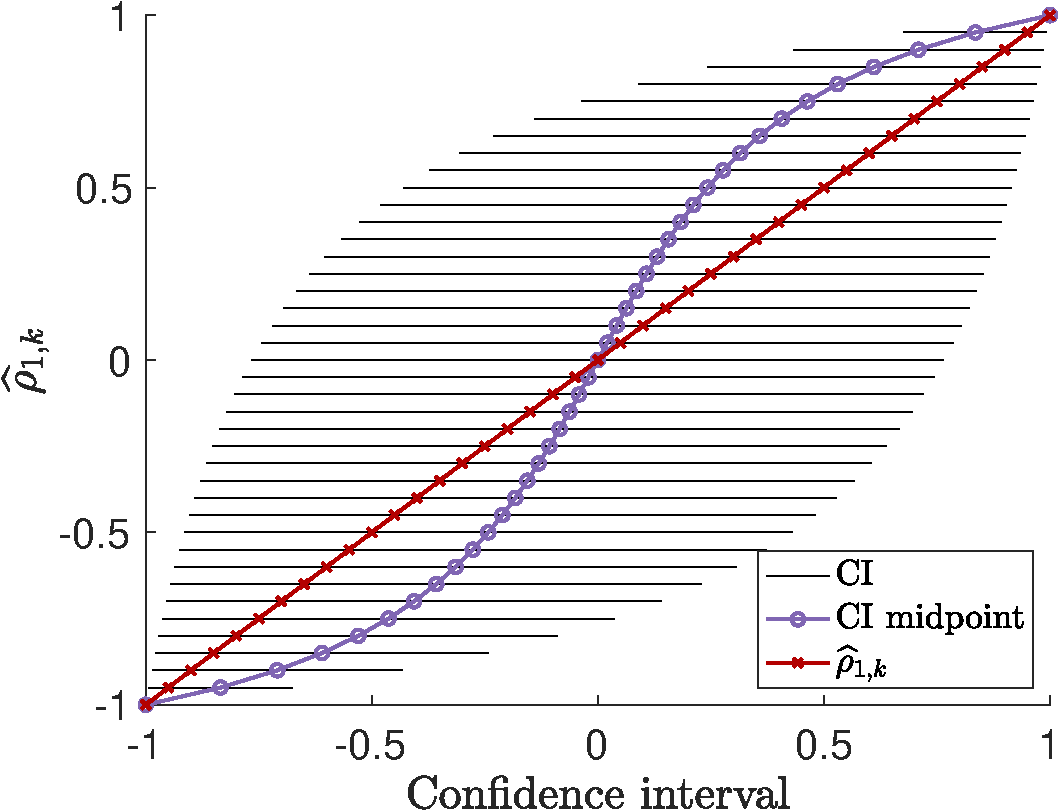
\includegraphics[width=0.3\linewidth]{./figures/CI_Q_5.pdf}&
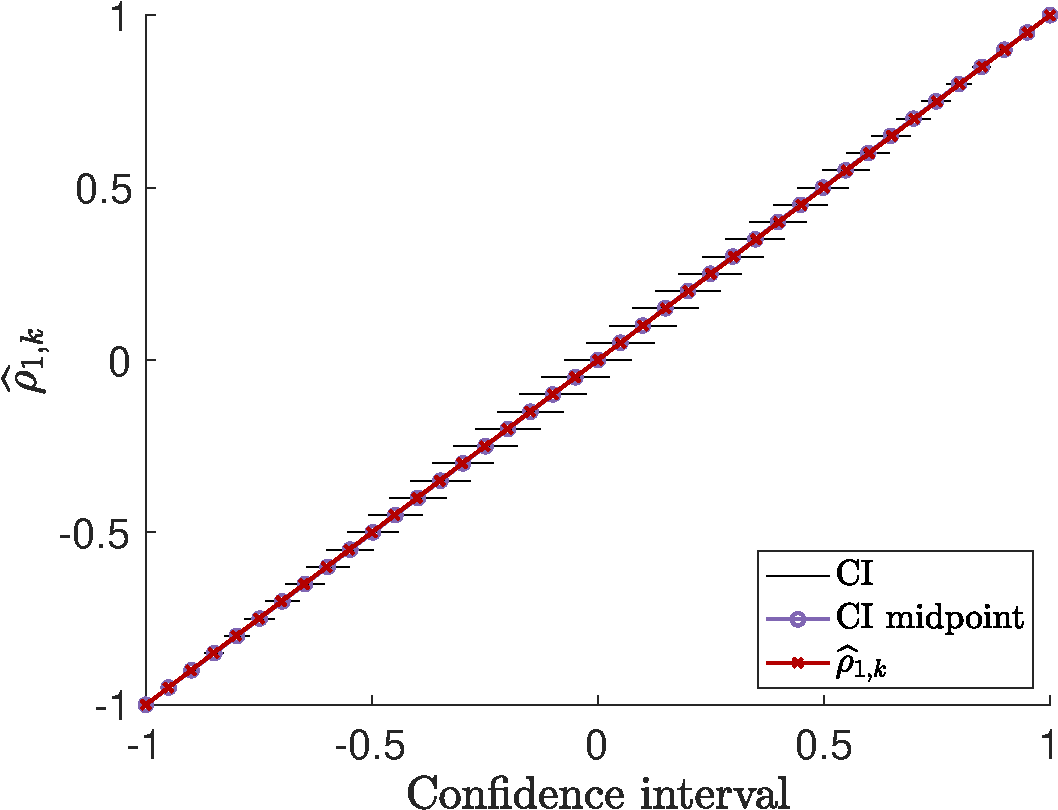
\includegraphics[width=0.3\linewidth]{./figures/CI_Q_30.pdf}&
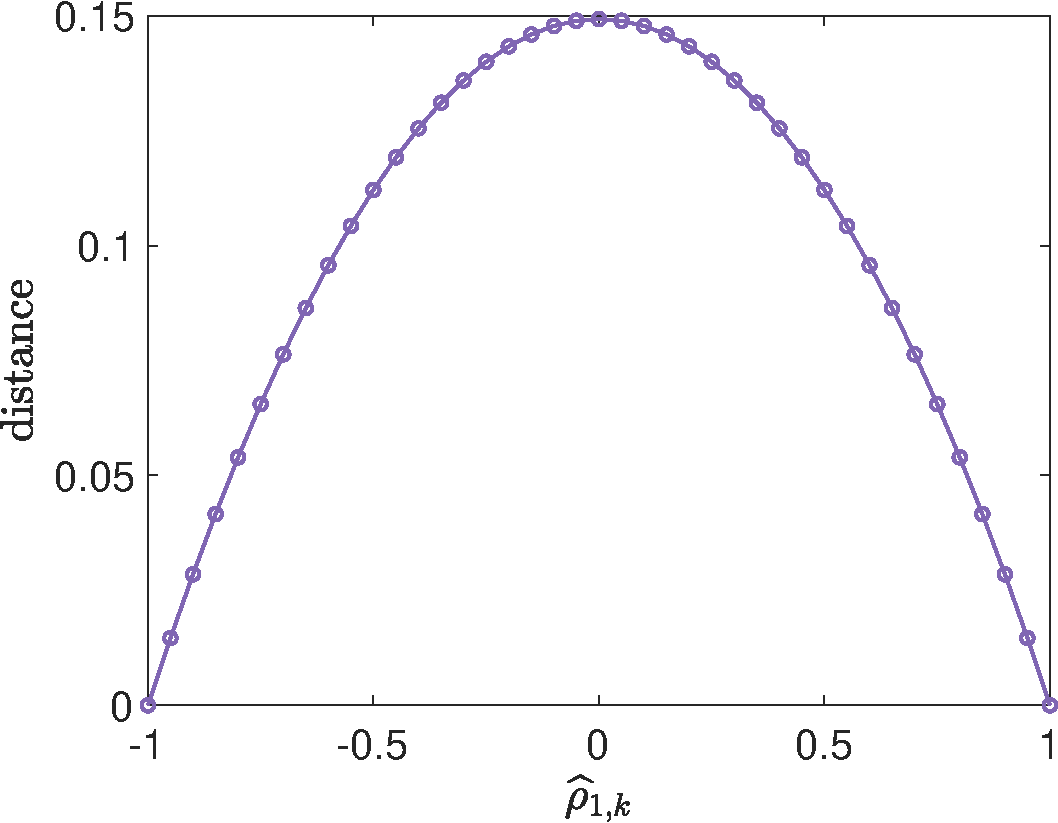
\includegraphics[width=0.3\linewidth]{./figures/CI_distance.pdf}
\end{tabular}
\caption{Left: confidence interval for $\rho_{1,k}$ with $Q=5$. Middle: confidence interval for $\rho_{1,k}$ with $Q=30$. Right: length of confidence interval for $Q=30$. It is an even function in terms of $\widehat \rho_{1,k}$. All plots are generated with $\widehat \rho_{1,k}=-1+0.05t$ with $t=0,\ldots,40$. 95\% confidence interval with $z_{\alpha/2}=1.96$.} 
\label{fig:CI_plot} 
\end{figure}
%

This confidence interval, together with the sensitivity analysis, forms the basis of a robust stopping rule for adaptive sampling. Specifically, we determine the minimal pilot sample size $Q$ required for reliable parameter estimation by sequentially updating sample statistics as $Q$ increases \cite{La:2001,Wa:1947}. Sampling continues until both accuracy and confidence criteria are satisfied. This adaptive strategy is summarized in Algorithm~\ref{algo:Parameter_Estimation} and is integrated into the enhanced model selection procedure described in Section~\ref{sec:Model_Selection} (Algorithm~\ref{algo:enhanced_mfmc_selection}).
%
\begin{algorithm}[!ht]
\DontPrintSemicolon

    \KwIn{Tolerance $\delta$, splitting ratio $\theta_1 = 0.5$, number of low-fidelity model $K$, initial sample size $Q_0$, sample size correction $dQ = Q_0$. Initializations for Welford's algorithm: proxies of mean, variance and covariance of high- and low-fidelity models $\widehat m_1^{(0)} = 0, \widehat m_k^{(0)} = 0$, $\widehat v_1^{(0)}=0, \widehat v_k^{(0)}=0$, $\widehat r_k^{(0)}=0$.}
    \KwOut{Sample size $Q$ for dynamic sampling, estimated parameters $\sigma_1,\alpha_k, \boldsymbol{\rho}$, cost efficiency $\xi$.}

    
    $\text{AddSample = True}.$

    $p=0, \xi^{(p)} = 0.$
    
    \While{AddSample = True}{
    
    \For{$k=2,\ldots, K$}{
    
        \For{$i = 1,\cdots, dQ $}
    {
    $j=p+i$.
    
    Estimate sample means $\widehat m_1^{(j)}, \widehat m_k^{(j)}$, standard deviations $\widehat\sigma_1^{(j)}, \widehat\sigma_k^{(j)}$, covariances $\widehat{\text{Cov}}^{(j)}$ and correlated coefficients $\widehat\rho_{1,k}^{(j)}$ by Welford's algorithm.
    }
    }
    % [$\text{index},\xi^{(p)}$] = Multi-fidelity Model Selection ($\boldsymbol{\rho}^{(p)},\boldsymbol{C}$).
    
    
    [$\text{index},\xi^{(p+dQ)}$] = Multi-fidelity Model Selection ($\widehat{\boldsymbol{\rho}}^{(p+dQ)},\boldsymbol{C}$).

    

    % Using selected models, estimate pilot sample size $Q_t$ via \eqref{eq:Offline_Sample_Size}.
    
    % Compute  $\xi^{(j)}$ by \eqref{eq:MFMC_sampling_cost_efficiency} with the selected $K^*$ models.
    
    
    \If{$\max\left\{\left|\frac{\xi^{(p+dQ)}-\xi^{(p)}}{\xi^{(p+dQ)}}\right|, \left|\frac{\mathbb{V}\left[A^{\text{MF}}\right]^{(p+dQ)}-\mathbb{V}\left[A^{\text{MF}}\right]^{(p)}}{\mathbb{V}\left[A^{\text{MF}}\right]^{(p+dQ)}}\right|\right\}<\delta$}
    % $\&$ $\left|\frac{\sigma_{k}^{(j)}-\sigma_{k}^{(j-1)}}{\sigma_{k}^{(j)}}\right|<\delta$ $\&$ $\left|\frac{\widehat \sigma_{k}^{(j)}-\widehat \sigma_{k}^{(j-1)}}{\widehat \sigma_{k}^{(j)}}\right|<\delta$ for all $k=2,\ldots, K$}
    {

    Using \eqref{eq:delta_xi_bound} and \eqref{eq:delta_var_bound} to compute threshold $\delta_1 = 2\delta/(A \sqrt{K^* - 1})$ for $\boldsymbol{\rho}$.
    
    Compute $z_k$ and the confidence interval $\text{CI}_{\rho_{1,k}}$ as in \eqref{eq:Fisher_z} and \eqref{eq:Confidence_Interval_rho}.
    

    
    \If{ the length of confidence interval is bigger than $\delta_1$}
    {
    \text{AddSample = False.}
    }
    \Else {
    \text{AddSample = True.}
    }
    }
    \Else {
    \text{AddSample = True.}
    
    $\xi^{(p)} = \xi^{(p+dQ)}$.
    
     $p=p+dQ$.}
    
    % \If{$j<Q_t$}
    % {
    % AddSample = True
    % }
    
    }    
    
    $Q=j$, $\sigma_1 = \widehat\sigma_1^{(j)}(\text{index})$, $\sigma_k = \widehat\sigma_k^{(j)}(\text{index})$, $\boldsymbol{\rho} = \widehat{\boldsymbol{\rho}}^{(j)}(\text{index})$.
\caption{Dynamic strategy for parameter estimation}\label{algo:Parameter_Estimation}
\end{algorithm}


\subsection{Model selection}\label{sec:Model_Selection}
After obtaining the confidence interval \eqref{eq:Confidence_Interval_rho} for correlation coefficients $\{\rho_{1,k}\}_{k=1}^{K}$, we want to select the correlation coefficient to meet the criterion of the Theorem \ref{thm:Sample_size_est}. The issue occurs when the confidence interval of correlation coefficients may overlap, as shown in Figure \ref{fig:CI_plot}. Overlapping confidence intervals does not directly mean that there is no significant difference in the parameters, and requires hypothesis testing or more precise confidence interval analysis. The following two methods select the model with correlations satisfy the two conditions in Theorem \ref{thm:Sample_size_est}. 
\newline 

\noindent {\bf Bootstrap method}
This method does not consider the distribution and is thus flexible, but may suffer from extra sampling cost. Repeatedly sample for $B$ times, create a sample statistics with Bootstrap method. For condition (i) of Theorem \ref{thm:Sample_size_est}, let $H_0:$ there was no significant difference in adjacent correlation coefficients (i.e. $|\rho_{1,k}|\le |\rho_{1,k+1}|$). $H_1:$ correlation coefficients decrease significant (i.e. $|\rho_{1,k}|> |\rho_{1,k+1}|$).  Estimate $|\widehat \rho_{k}^{(b)}|$ and $|\widehat \rho_{k+1}^{(b)}|$. Then estimate the $1-\alpha$ confidence interval for $|\widehat \rho_{k}^{(b)}| - |\widehat \rho_{k+1}^{(b)}|$. If the lower bound of the confidence interval is positive, then reject $H_0$ and accept $H_1$, and vice versa. If $H_1$ is accepted, then remove the model with $\widehat \rho_{1,k}$, since it has a larger cost. For condition (ii) of Theorem \ref{thm:Sample_size_est}, estimate $
D_k^{(b)} = C_{k-1}((\widehat\rho_{1,k}^{(b)})^2-(\widehat \rho_{1,k+1}^{(b)})^2)-C_k((\widehat\rho_{1,k-1}^{(b)})^2-(\widehat \rho_{1,k}^{(b)})^2)$, and compute its corresponding $1-\alpha$ confidence intervals. If the lower bound of the confidence interval is positive, then the second condition (ii) holds. Finally, accept the confidence interval with $\widehat \rho_{1,k+1}$ for $k\ge 1$.
\newline 

\noindent {\bf Transformation based method}
For condition (i) of Theorem \ref{thm:Sample_size_est}, Under normality of the transformed variable $z_k$ and $z_{k+1}$ as in \eqref{eq:Fisher_z}, we first observe that tanh function is increasing with argument range from 0 to 1, therefore consider 
\[
\left|\widehat \rho_{1,k}\right| = \text{tanh}(|z_k|), \quad D = \left|\widehat \rho_{1,k}\right|-\left|\widehat \rho_{1,k+1}\right|=\text{tanh}(|z_k|)-\text{tanh}(|z_{k+1}|)
\]
Consider Delta approximation (first order Taylor approximation) to D, we yield
\[
D\approx\frac{\partial D}{\partial Z_k}(z_k-\mu_{z_k})+\frac{\partial D}{\partial Z_{k+1}}(z_{k+1}-\mu_{z_{k+1}}),
\]
where $\frac{\partial D}{\partial Z_k} = \text{sign}(z_k)4e^{2|z_k|}/(e^{2|z_k|}+1)^2$ and $\mu_{z_k}$ is the expected value.  And the variance of $D$ is
\[
\text{Var}(D) \approx \left(\frac{\partial D}{\partial z_k}\right)^2 \text{Var}(z_k)+\left(\frac{\partial D}{\partial z_{k+1}}\right)^2 \text{Var}(z_{k+1})+2 \frac{\partial D}{\partial z_k} \frac{\partial D}{\partial z_{k+1}}\text{Cov}(z_k,z_{k+1})=\frac{1.06}{Q-3}\left[\frac{16e^{4|z_k|}}{(e^{2|z_k|}+1)^4} +\frac{16e^{4|z_{k+1}|}}{(e^{2|z_{k+1}|}+1)^4}\right]
\]
Note that since $z_k$ and $z_{k+1}$ are independent, then the covariance term becomes 0 and after the Fisher transformation and its exact variance is known as $\sigma_{z_k} = 1.03/\sqrt{Q - 3}$.

We will consider t test (Student t-test) to determine whether there is a significant difference between the means of two groups of samples, especially for our case, to determine if  $| \rho_{1,k}|$ and $|\rho_{1,k+1}|$ have a significant difference  with overlapping confidence intervals. The assumption for t test requires at least approximately normal distribution for sample means, this does not hold since the transformed statistic $D$ is in general not approximately normal, unless $Q>30$ and $\widehat \rho_{1,k}$ stays away from $\pm 1$. Consider independent two-sample t-test statistic
% We consider independent two-sample t-test. 



\[
t = \frac{D}{\sqrt{\text{Var}(D)}} \sim t_\nu, \quad \nu = Q-3
\]
where $t_\nu$ is a t distribution  with degrees of freedom of $\nu = Q-3$. If $t>t_{\alpha,\nu}$, where $t_{\alpha,\nu}$ is a value in the t distribution table,  we reject $H_0$, we think $\widehat \rho_{1,k}$ is obvious larger than $\widehat \rho_{1,k+1}$. Otherwise, $|\widehat \rho_{1,k}|$ is very close to $|\widehat \rho_{1,k+1}|$, in this scenario, we will discard the model with $|\widehat \rho_{1,k}|$ and keep the model with $|\widehat \rho_{1,k+1}|$.

% If sample variances are similar in the sense that $0.5<\sigma_{z_k}^2/\sigma_{z_{k+1}}^2<2$, the corresponding $t$ statistic is
% \[
% t_k=\frac{D}{s_p\sqrt{\frac{1}{Q_1}+\frac{1}{Q_2}}}, \quad s_p = \sqrt{\frac{(Q_1 - 1)\sigma_{z_k}^2 + (Q_2 - 1)\sigma_{z_{k+1}}^2}{Q_1+Q_2-2}}
% \]
% Otherwise,

% \[
% t_k = \frac{\Delta z_k}{\sqrt{\frac{\sigma_{z_k}^2}{Q_1} + \frac{\sigma_{z_{k+1}}^2}{Q_2}}}
% \]







For condition (ii) of Theorem \ref{thm:Sample_size_est}, consider
\[
E = -C_{k}\widehat \rho_{1,k-1}^2+(C_{k-1} + C_k)\widehat\rho_{1,k}^2  - C_{k-1}\widehat\rho_{1,k+1}^2 =-C_{k}\text{tanh}^2(z_{k-1}) + (C_{k-1} + C_k)\text{tanh}^2(z_{k})-C_{k-1}\text{tanh}^2(z_{k+1})
\]
we want to check if $E>0$ holds or not. 
%
\begin{align*}
    E &\approx \sum_{i=k-1}^{k+1}\frac{\partial E}{\partial z_i}(z_i-\mu_{z_i})
\end{align*}
%
where
\begin{equation*}
    \frac{\partial E}{\partial z_i}= \left\{\begin{array}{ll}
-2C_k\text{tanh}(z_{k-1})\text{sech}^2(z_{k-1}), & i=k-1,\\
2(C_{k-1} + C_k)\text{tanh}(z_{k})\text{sech}^2(z_{k}), & i=k,\\
- 2C_{k-1}\text{tanh}(z_{k+1})\text{sech}^2(z_{k+1}), & i=k+1.
\end{array}
\right.
\end{equation*}


with variance
\[
\text{Var}(E)\approx \sum_{i=k-1}^{k+1}\left(\frac{\partial E}{\partial z_i}\right)^2 \text{Var}(z_i) + 2\sum_{i<j}\frac{\partial E}{\partial z_i}\frac{\partial E}{\partial z_j}\text{Cov}(z_i,z_j)
\]
Note that since $z_{k-1}$, $z_k$ and $z_{k+1}$ are independent, then the covariance term becomes 0. Consider
\[
t=\frac{E}{\sqrt{\text{Var}(E)}} \sim t_\nu, \quad \nu = Q-3
\]
If $t>t_{\alpha,\nu}$, we accept accept $E>0$, namely the second condition (ii) holds.


% If no normality is assumed, we consider the two successive level $k$ and $k+1$, and consider the worst square difference
% \begin{equation}
% \label{eq:delta_rho_square}
%     \Delta_k^{\text{min}} = \max \left\{\left(\rho_{1,k}^{\text{lower}}\right)^2 - \left(\rho_{1,k+1}^{\text{upper}}\right)^2,0\right\},\quad \Delta_k^{\text{max}} = \left(\rho_{1,k}^{\text{upper}}\right)^2 - \left(\rho_{1,k+1}^{\text{lower}}\right)^2,
% \end{equation}
% where $\rho_{1,1}^{\text{lower}} =\rho_{1,1}^{\text{upper}}= 1, \rho_{1,K+1}^{\text{lower}}=\rho_{1,K+1}^{\text{upper}} = 0$. If $\Delta_k^{\text{min}}=0$, it indicates that level $k$ and $k+1$ may encounter overlap and does not have obvious distinction, we could consider to combine these two levels. Moreover, if uncertainty is small and confidence interval is almost symmetric, we believe that the true value is most likely to fall near the middle of the interval $\overline{\rho}_{1,k} = \frac{1}{2}(\rho_{1,k}^{\text{lower}}+\rho_{1,k}^{\text{upper}})$, we can consider the midpoint of each confidence interval (instead of two endpoints) and substitute into \eqref{eq:delta_rho_square}.




% %
% \begin{equation*}\label{eq:Optimization_pb_model_selection}
%     \begin{array}{lll}
%     \displaystyle\min_{S^*} &\displaystyle \xi,\\
%        \text{s.t.} &\displaystyle |\rho_{1,1}|>\ldots>|\rho_{1,K^*}|,\\
%        &\displaystyle \frac{C_{i-1}}{C_i}>\frac{\rho_{1,i-1}^2-\rho_{1,i}^2}{\rho_{1,i}^2-\rho_{1,i+1}^2}, \quad i=1,\ldots,{K^*}, \quad \rho_{1,K^*+1}=0,\\
%     \end{array}
% \end{equation*}
% %

% \normalem
% \begin{algorithm}[!ht]
% \label{algo:MFMC_Algo_model_selection}
% \DontPrintSemicolon    
%    \KwIn{$K$ candidate models $\widehat  u_{h, k}$ with coefficients $\rho_{1,k}$, $\sigma_1$, $\sigma_k$ and cost per sample $C_k$.}\vspace{1ex}
    
%     \KwOut{Selected $K^*$ models $\widehat u_{h, i}$ in $\mathcal{S}^*$, with coefficients $\rho_{1,i}$, $\alpha_i$ and $C_i$ for each model $\widehat u_{h, i}$.}\vspace{1ex}
%     \hrule \vspace{1ex}

%    % Estimate $\rho_{1,k}$ and $C_k$ for each model $u_{h, k}$ using $N_0$ samples.
   
   
%    Sort $u_{h, k}$ by decreasing $\rho_{1,k}$ to create $\mathcal{S}=\{\widehat u_{h, k}\}_{k=1}^K$. 
   
%    Initialize $w^*=C_1$, $\mathcal{S}^*=\{\widehat u_{h, 1}\}$. Let $ \mathcal{\widehat S}$ be all $2^{K-1}$ ordered subsets of $\mathcal{S}$, each containing $\widehat u_{h, 1}$. 
%    % Set $ \mathcal{\widehat S}_1=\mathcal{S}^*$.

%     % $(2 \le j \le 2^{K-1})$
%     \For{each subset $\mathcal{\widehat S}_j$\,}{

%     {
%     \If{ condition $(ii)$ from Theorem \ref{thm:Sample_size_est} is satisfied}{
%     Compute the objective function value $w$ using \eqref{eq:MFMC_sampling_cost_efficiency}.
    
%     \If{$w<w^*$}{
%     {
%     Update $\mathcal{S}^* = \mathcal{\widehat S}_j$ and $w^* = w$.
%     }
%     } 
%     }
%     }
%     $j=j+1$.
%     }
%     Compute $\alpha_i$ for $\mathcal{S}^*$, $i=2,\dots, K^*$ by \eqref{eq:MFMC_coefficients}.
% \caption{Multi-fidelity Model Selection--\JLcolor{\cite[Algorithm~1]{PeWiGu:2016}}}
% \end{algorithm}
% \ULforem


\normalem
\begin{algorithm}[!ht]
\label{algo:enhanced_mfmc_selection}
\DontPrintSemicolon
\SetAlgoVlined
\SetKwProg{Fn}{Function}{}{}
\SetKwInOut{Input}{Input}
\SetKwInOut{Output}{Output}

\Input{%
Vectors of correlation coefficients $\boldsymbol{\rho}$, costs per sample $\boldsymbol{C}$, sample deviations $\boldsymbol{\sigma}$. 
}
\Output{%
  Set of selected models $\mathcal{S}^*=\{u_{h,i}\}_{i\in I^*}$, correlations of selected models $\boldsymbol{\rho}^*$, costs of selected models $\boldsymbol{C}^*$, minimal cost efficiency ratio $\xi_{\text{min}}$, weights $\alpha_i^*$.
}
\hrule
 
\Fn{[idx\textunderscore for\textunderscore model, $\xi_{\text{min}}$] = Model\textunderscore Selection\textunderscore Backtrack ($\boldsymbol{\rho}, \boldsymbol{C}$)}{
Sort the correlation coefficients by non-increasing $|\rho_{1,k}|$ with order $r$. Relabel $\rho_{1,k}, C_k$ for all $k$ as $\boldsymbol{\rho}, \boldsymbol{C}$.


Initialization: 
current$\_$idx = 1, $\xi_{\text{min}}=1$, global$\_$idx = []. %$\boldsymbol{\rho}=[1]$, $\boldsymbol{C}=[C_1]$,


\vspace{3mm}
\textbf{Backtrack} $(\text{current}\_\text{idx},\, \xi_{\text{min}},\, 2)$. 

idx\textunderscore for\textunderscore model = r(global$\_$idx).
\vspace{3mm}

\Fn{ $[\mathcal{S}^*,\, \boldsymbol{\rho}^*, \,\boldsymbol{C}^*, \xi_{\text{min}}]$ = \textbf{Backtrack} $\left(\text{current}\_\text{idx}, \, \xi, \,k_{\text{next}}\right)$}{


  \If{$\xi \leq \xi_{\text{min}}\,$ }{
    $\xi_{\text{min}}=\xi$.

    global$\_$idx = current$\_$idx.
  }
  % \Else {
  %   $\mathcal{S}^* = \mathcal{S}$, $\boldsymbol{\rho}^* = \boldsymbol{\rho}$, $\boldsymbol{C}^* = \boldsymbol{C}$, $\xi_{\text{min}}=\xi$.
  % }
  
  \If{$k_{\text{next}} > K$}{ 
    \Return
  }
  
  \For{$k = k_{\text{next}}$ \textbf{to} $K$}{ 
     % $\rho_{1,\text{last}} = \boldsymbol{\rho}_{\text{end}}$, $C_{\text{last}} = \boldsymbol{C}_{\text{end}}$.
     previous\textunderscore idx = current$\_$idx (end).

     % $\rho_k = \boldsymbol{\rho}(k), C_k = \boldsymbol{C}(k)$

     % $\rho_{\text{next}}=0$

     
    \If{% 
      $\frac{\boldsymbol{C}({\text{previous}\_\text{idx}})}{\boldsymbol{C}(k)} > \frac{\boldsymbol{\rho}({\text{previous}\_\text{idx}})^2 - \boldsymbol{\rho}(k)^2}{\boldsymbol{\rho}(k)^2}$ 
    }{
        Continue to next iteration.
    }

        % $\rho_k\_$vec = [$\boldsymbol{\rho}$(cur$\_$ind), $\rho_k$]
        
        Compute $\xi$ via \eqref{eq:MFMC_sampling_cost_efficiency} for indices  
      [current\textunderscore idx, $k$].

      \If{$\xi\ge \xi_{\text{min}}$ or $\,\xi>1$}{ 
    Continue to next iteration.
    }
      
      \textbf{Backtrack} $(\, [\text{current}\_\text{idx},k],\xi, k+1)$.
  }
}
}
\vspace{3mm} 


 
$I^* = \text{idx}\_\text{for}\_\text{model}, K^* = |I^*|, \boldsymbol{\rho}^* = \boldsymbol{\rho} (I^*)$, $\boldsymbol{C}^* = \boldsymbol{C} (I^*)$, $\boldsymbol{\sigma}^* = \boldsymbol{\sigma} (I^*)$.

Selected models $\mathcal{S}^* = \{u_{h,k}\}_{k\in \mathcal{I^*}}$ with weights $\alpha_i^*$ for $i=2,...,K^*$ via \eqref{eq:MFMC_SampleSize}.




\caption{Multi-fidelity Model Selection with Backtracking Pruning}
\end{algorithm}
\ULforem




\normalem
\begin{algorithm}[!ht]
\label{algo:MFMC_Algo}
\DontPrintSemicolon

    
   \KwIn{Selected $K^*$ models $u_{h, k}$ in $\mathcal{S}^*$, parameters $\rho_{1,k}$, $\alpha_k$ and $C_k$ for each $u_{h, k}$,  tolerance $\epsilon$. }\vspace{1ex}
    
    \KwOut{Sample sizes $N_k$ for $K^*$ models, expectation 
    estimate $A^{\text{MF}}$.}\vspace{1ex}
    \hrule \vspace{1ex}
    

    Compute the sample size $N_k$ for $1\leq k\leq K^*$ by \eqref{eq:MFMC_SampleSize} and generate i.i.d. $N_1$ and $N_k-N_{k-1}$ samples for $k=2,\ldots, K^*$.

    Evaluate $u_{h, 1}$ to obtain $u_{h, 1}(\boldsymbol{\omega}^i)$ for $i = 1,\ldots,N_1$ and compute $A_{1,N_1}^{\text{MC}}$ by \eqref{eq:MC_estimator}.
    
    \For{$k = 2,\ldots,K^* $\,}{

    Evaluate $u_{h, k}$ to obtain $u_{h, k}(\boldsymbol{\omega}^i)$ for $i = 1,\ldots,N_{k-1}$ and compute $A_{k,N_{k-1}}^{\text{MC}}$ by \eqref{eq:MC_estimator}.

    Evaluate $u_{h, k}$ to obtain $u_{h, k}(\boldsymbol{\omega}^i)$ for $i = 1,\ldots,N_k-N_{k-1}$ and compute $A_{k,N_k\backslash N_{k-1}}^{\text{MC}}$ by \eqref{eq:MC_estimator}.

    % Store $N_{k-1}$ and $N_{k}-N_{k-1}$ samples as $N_k$ samples.
    }

    Compute $A^{\text{MF}}$ by \eqref{eq:MFMC_estimator_independent}.
    
\caption{Multifidelity Monte Carlo}
\end{algorithm}
\ULforem

% \normalem
% \begin{algorithm}[!ht]
% \label{algo:MFMC_Algo}
% \DontPrintSemicolon

    
%    \KwIn{Models $f_k$ in $\mathcal{S}^*$, parameters $\rho_k$, $\alpha_k$ and $C_k$ for each $f_k$ in $\mathcal{S}^*$,  tolerance $\epsilon$. }\vspace{1ex}
    
%     \KwOut{Sample sizes $N_k$ for $K^*$ models, expectation 
%     estimate $A^{\text{MFMC}}$.}\vspace{1ex}
%     \hrule \vspace{1ex}
%     Compute initial sample sizes $\boldsymbol{N}=[N_1,\ldots, N_{K^*}]$ using \eqref{eq:MFMC_SampleSize}. Set $\boldsymbol{N}_{\text{old}} = \boldsymbol{0}$ and $\boldsymbol{dN} = \boldsymbol{N}$. 
    
%     Initialize sample means $A_{1,N_1}^{\text{MC}}, A_{k,N_{k-1}}^{\text{MC}}, A_{k,N_k\backslash N_{k-1}}^{\text{MC}}=0. $
    
%     \While{$\sum_k dN_k>0$\,}{

%     Evaluate $dN_{1}$ samples for $f_1$ to obtain $f_1(\boldsymbol{\omega}^i)$. Update $A_{1,N_1}^{\text{MC}} = \frac{\boldsymbol{N}_{\text{old}}^1 A_{1,N_1}^{\text{MC}}+\sum_i f_1(\boldsymbol{\omega}^i)}{\boldsymbol{N}_{\text{old}}^1+dN_1}$ and $\sigma_1$.

%     Store $dN_1$ samples.
    
%     \For{$2\le k\le K^*$\,}{
    
%         % \For{$i = 1,\ldots,dN_k $\,}
%     % {
%     Evaluate previously stored $dN_{k-1}$ samples for $f_k$ to obtain $f_k(\boldsymbol{\omega}^i)$. Update $A_{k,N_{k-1}}^{\text{MC}} = \frac{\boldsymbol{N}_{\text{old}}^k A_{k,N_{k-1}}^{\text{MC}}+\sum_i f_k(\boldsymbol{\omega}^i)}{\boldsymbol{N}_{\text{old}}^k+dN_{k-1}}$. 
    
%     Collect new $dN_{k}-dN_{k-1}$ samples. Evaluate $f_k$ to obtain $f_k(\boldsymbol{\omega}^i)$. Update $A_{k,N_k\backslash N_{k-1}}^{\text{MC}} = \frac{\boldsymbol{N}_{\text{old}}^k A_{k,N_k\backslash N_{k-1}}^{\text{MC}}+\sum_i f_k(\boldsymbol{\omega}^i)}{\boldsymbol{N}_{\text{old}}^k+dN_{k}-dN_{k-1}}$. 

    
%     Compute $\sigma_k, \rho_{1,k}$.

%     Store $dN_{k-1}$ and $dN_{k}-dN_{k-1}$ samples as $dN_k$ samples.
    
%     \If{Condition (i) \& (ii) in Theorem \ref{thm:Sample_size_est} is not satisfied \,}{
%     Reselect models via Algorithm \ref{algo:MFMC_Algo_model_selection} with a larger sample size and restart.

%     Break. 
%     }

%     }
    
    
    
%     \vspace{4mm}
%     $\boldsymbol{N}_{\text{old}} \leftarrow \boldsymbol{N}$
    
%     Update $\alpha_k$ and the sample size $\boldsymbol{N}$ by \eqref{eq:MFMC_coefficients} 
%  and \eqref{eq:MFMC_SampleSize}.

%     $\boldsymbol{dN} \leftarrow \max \left\{\boldsymbol N-\boldsymbol N_{\text{old}}, \boldsymbol{0}\right\}.$

    
%     }
%     Compute $A^{\text{MFMC}}$ using $A_{1,N_1}^{\text{MC}}, A_{k,N_{k-1}}^{\text{MC}}, A_{k,N_k\backslash N_{k-1}}^{\text{MC}}$ and $\alpha_k$ from step 4, 7, 8, 15, by \eqref{eq:MFMC_estimator_independent}.
% \caption{Multi-fidelity Monte Carlo}
% \end{algorithm}
% \ULforem


% \begin{theorem}
% \label{thm:Sampling_cost_est}
% Let $f_k$ be $K$ models that satisfy the following conditions
% %
% \begin{alignat*}{8}
%     &(i)\;\; |\rho_{1,1}|>\ldots>|\rho_{1,K}|& \qquad \qquad
%     &(ii)\;\; \frac{C_{k-1}}{C_k}>\frac{\rho_{1,k-1}^2-\rho_{1,k}^2}{\rho_{1,k}^2-\rho_{1,k+1}^2},\;\;k=2,\ldots,K.
% \end{alignat*}
% %
% Suppose there exists $0<s<q<1$ such that 
% $C_k = c_s s^{k}$, $\rho_{1,k}^2 = q^{ k-1}$, then 
% \begin{equation*}
%     \mathcal{W}_\text{MFMC} = 
% \end{equation*}

% \end{theorem}
% \begin{proof}
% Since $q>s$, condition (ii) is satisfied.
% \begin{align*}
% \rho_{1,k}^2 - \rho_{1,k+1}^2&=q^k\left(\frac1 q-1\right),\quad \rho_{1,k-1}^2 - \rho_{1,k}^2=q^k\frac 1 q\left(\frac1 q-1\right)\\
%     \mathcal{W}_\text{MFMC} &= \frac{\sigma_1^2}{\left\Vert\mathbb{E}(f_1) \right\Vert_{Z}^2\epsilon^2}\sum_{k=1}^K\sqrt{\left(\rho_{1,k}^2 - \rho_{1,k+1}^2\right)C_k}\sum_{k=1}^K\left(\sqrt{\frac{C_k}{\rho_{1,k}^2 - \rho_{1,k+1}^2}} - \sqrt{\frac{C_{k-1}}{\rho_{1,{k-1}}^2 - \rho_{1,k}^2}}\right)\rho_{1,k}^2,\\
%     &=\frac{\sigma_1^2}{\left\Vert\mathbb{E}(f_1) \right\Vert_{Z}^2\epsilon^2} \sum_{k=1}^K\sqrt{q^{k}s^{ k}}\left(\sqrt{\frac{s(1-q)}{1-\rho_{1,2}^2}} + \sum_{k=2}^K\left(\sqrt{\frac{s^{k}}{q^{ k}}} - \sqrt{\frac{q s^{ k}}{s q^{ k}}}\right)q^{k} + \left(\sqrt{\frac{s^{ K}(1-q)}{q^{K}}}-\sqrt{\frac{q s^{ K}}{s q^{K}}}\right)q^{K}\right)\\
%     &\propto \frac{1}{\epsilon^2} \sum_{k=1}^K\left(q^{\frac{1}{2}}s^{\frac{1}{2}}\right)^k
% \end{align*}
    
% \end{proof}


%
\subsection{Confidence interval for sample size and total cost}
Given the confidence intervals $\text{CI}_{\rho_{1,k}}$ for the correlation coefficients as defined in \eqref{eq:Confidence_Interval_rho}, we aim to derive the corresponding confidence intervals $\text{CI}_{N_k}$ for the required sample sizes in the multi-fidelity Monte Carlo estimator. 

% This involves solving an optimization problem that minimizes the total computational cost while satisfying an upper bound on the estimator variance and enforcing monotonicity constraints on the sample sizes. 
%
\begin{theorem}
\label{thm:Sample_size_est_conf_interval} 
Let $\text{CI}_{\rho_{1,k}}$ be the confidence interval for the estimated correlation coefficient as defined in \eqref{eq:Confidence_Interval_rho}, and let $N_k^*$ denote the optimal sample size from \eqref{thm:Sample_size_est}. Define the lower and upper bounds for the sample size
%
\begin{equation}\label{eq:upper_lower_N_k}
    N_k^{\text{lower}} = \frac{\sigma_1^2}{\epsilon_{\text{tar}}^2}\sqrt{\frac{\Delta_k^{\min}}{C_k}}\sum_{j=1}^K\sqrt{C_j\Delta_j^{\min}},\quad N_k^{\text{upper}} = \frac{\sigma_1^2}{\epsilon_{\text{tar}}^2}\sqrt{\frac{\Delta_k^{\max}}{C_k}}\sum_{j=1}^K\sqrt{C_j\Delta_j^{\max}}
\end{equation}


%
Then the confidence interval for $N_k$ is
%
\[
\text{CI}_{N_k} = \left[N_k^*-1.96\sqrt{\text{Var}\left[N_k\left(\widehat\rho_{1,k}\right)\right]}, N_k^*+1.96\sqrt{\text{Var}\left[N_k\left(\widehat\rho_{1,k}\right)\right]}\right]\cap \left[N_k^{\text{lower}}, N_k^{\text{upper}}\right].
\]
%
\end{theorem}

\begin{proof}



% \[
% \overline{\rho}_{1,k} = \frac{\rho_{1,k}^{\text{lower}}+\rho_{1,k}^{\text{upper}}}{2}, \quad \Delta_k = \max \left\{\overline{\rho}_{1,k}^2 - \overline{\rho}_{1,k+1}^2,0\right\},
% \]
% we consider the constrained optimization problem \ref{eq:Optimization_pb_sample_size}
% %
% \begin{equation}\label{eq:Optimization_pb_sample_size2}
%     \begin{array}{ll}
%     \min \limits_{\begin{array}{c}\scriptstyle N_1,\ldots, N_K\in \mathbb{R} \\[-4pt]
% \end{array}} &\displaystyle\sum\limits_{k=1}^K C_kN_k,\\
%        \;\,\text{subject to} &\mathbb{V}\left[A^{\text{MF}}\right]=\sigma_1^2 \sum_{k=1}^K\frac{\rho_{1,k}^2 - \rho_{1,k+1}^2}{N_k}=   \epsilon_{\text{tar}}^2,\\[2pt]
%        &\displaystyle -N_1\le 0,\quad \displaystyle N_{k-1}-N_k\le 0, \;\; k=2\ldots,K.
%     \end{array}
% \end{equation}
% %
% Condition (ii) of Theorem \ref{thm:Sample_size_est} indicates that $S^\prime<0$ in \eqref{eq:S_n_S_prime}, therefore,  both $\mathbb{V}[A^{\text{MF}}]$ and optimal sample size $N_k$ are monotonically decreasing in  $\rho_{1,k}$ as shown in \eqref{eq:partial_var_rho}.  Thus, the largest sample size and variance occur at the lower confidence bounds $\widehat\rho_{1,k}^{\text{low}}$.

% To compute this upper bound on sample size, Substituting  $\rho_{1,k} = \widehat\rho_{1,k}^{\text{low}}$ into the variance constraint of \eqref{eq:Optimization_pb_sample_size2}, we solve the optimization problem with equality using Lagrange multipliers. The resulting Lagrangian is
% %
% \[
% L = \sum_{k=1}^K C_kN_k +\lambda_0 \left(\frac{\sigma_1^2}{N_1} - \sum_{k=2}^K \left(\frac{1}{N_{k-1}} - \frac{1}{N_k}\right)\left(\widehat\rho_{1,k}^{\text{low}}\right)^2\sigma_1^2\right)-\lambda_1 N_1+\sum_{k=2}^K\lambda_k(N_{k-1} - N_k),
% \]
% %
% Setting $\partial L / \partial N_k = 0$ yields the sample sizes $N_k^{\text{max}}$ as claimed.
% %
% \[
% N_k^{\text{max}} = \frac{\sigma_1^2}{\epsilon_{\text{tar}}^2}\sqrt{\frac{(\text{CI}_{\rho_{1,k}}^{\text{L}})^2-(\text{CI}_{\rho_{1,k+1}}^{\text{L}})^2}{C_k}}\sum_{j=1}^K\sqrt{C_j\left((\text{CI}_{\rho_{1,j}}^{\text{L}})^2-(\text{CI}_{\rho_{1,j+1}}^{\text{L}})^2\right)},\quad \text{for}\quad  k=1,\ldots,K.
% \]
% %

% At the upper endpoint $\widehat\rho_{1,k}^{\text{high}}$, the variance constraint is not active, and the optimal solution to the relaxed problem yields no meaningful lower bound (e.g., $N_k = 0$ is feasible). To obtain a practical confidence interval, we instead linearize $N_k$ with respect to $\rho_{1,k}$ using a first-order Taylor expansion:


% At the upper endpoint $\widehat\rho_{1,k}^{\text{high}}$, the variance constraint is strictly satisfied, and the corresponding Lagrange multiplier $\lambda_0$ vanishes due to complementary slackness. The optimization problem then reduces to minimizing the cost subject only to the non-decreasing sample sizes
% %
% \[
% \min \limits_{\begin{array}{c}\scriptstyle N_1,\ldots, N_K\in \mathbb{R}\end{array}}\sum\limits_{k=1}^K C_kN_k, \quad \text{subject to} \quad  0\le N_1\le \cdots \le N_K.
% \]
% %
% While the trivial solution $N_k^{\text{min}} = 0$ satisfies these constraints, it does not produce a meaningful lower bound. 

To obtain an informative characterization of the uncertainty in $N_k$, we linearize $N_k$ with respect to the estimated correlation $\widehat\rho_{1,k}$ using a first-order Taylor expansion
%
\[
 N_k\left(\widehat\rho_{1,k}\right)\approx N_k^*+ \frac{\partial N_k}{\partial \rho_{1,k}} \left( \widehat\rho_{1,k}-\rho_{1,k}\right).
\]
%
The variance of this linearized estimate is approximated by
%
\begin{align*}
    \text{Var}\left[N_k\left(\widehat\rho_{1,k}\right)\right] &\approx \left(\frac{\partial N_k}{\partial \rho_{1,k}}\Bigg |_{\rho_{1,k} = \widehat\rho_{1,k}} \right)^2 \cdot \text{Var}\left[\widehat\rho_{1,k}\right] \approx \left(\frac{\partial N_k}{\partial \rho_{1,k}}\Bigg |_{\rho_{1,k} = \widehat\rho_{1,k}} \right)^2 \cdot \left(\frac{\partial \text{tanh}(z)}{\partial z}\right)^2\text{Var}[z],\\
    &= \left(\frac{\partial N_k}{\partial \rho_{1,k}}\Bigg |_{\rho_{1,k} = \widehat\rho_{1,k}} \right)^2 \cdot \left(1-\widehat\rho_{1,k}^2\right)^2\frac{1.03^2}{Q-3}.
\end{align*}
%
This leads to a confidence interval for the linearized sample size estimate
%
\[
\text{CI}_{N_k} :=\left[N_k^*-1.96\sqrt{\text{Var}\left[N_k\left(\widehat\rho_{1,k}\right)\right]}, N_k^*+1.96\sqrt{\text{Var}\left[N_k\left(\widehat\rho_{1,k}\right)\right]}\right].
\]
%
Moreover, given $\rho_{1,k}\in \text{CI}_{\rho_{1,k}}$,   the sample size corresponding to \eqref{eq:delta_rho_square} is \eqref{eq:upper_lower_N_k}. Combining this with the linearized estimate yields the result.
\end{proof}

Finally, this range induces a confidence interval for the cost-efficiency metric $\xi$ introduced in \eqref{eq:MFMC_sampling_cost}, with bounds given by TOBEFINISHED.
% %
% \begin{equation}\label{eq:MFMC_sampling_cost_efficiency_CI}
%     \xi \in  \left[\sum_{k=1}^K C_k N_k^{\text{low}},\;\;\min \left\{\sum_{k=1}^K C_k N_k^{\text{high}},\frac{1}{C_1} \left(\sum_{k=1}^K\sqrt{C_k\left(\left(\rho_{1,k}^{\text{low}}\right)^2-\left(\rho_{1,k+1}^{\text{low}}\right)^2\right)}\right)^2\right\}\right].
% \end{equation}
% %

